\documentclass{beamer}

\usepackage[utf8]{inputenc}
\usepackage[croatian]{babel}
\usepackage[numbers, square]{natbib}

\newcommand{\engl}[1]{(engl.~\emph{#1})}
\setbeamertemplate{caption}[numbered]
\usetheme{Boadilla}

\title[Završni rad br. 5709]{Sustav za određivanje strukture teksta na temelju položaja pojedinih znakova}
\author{Herman Zvonimir Došilović}
\institute[FER]{Sveučilište u Zagrebu\\ Fakultet elektrotehnike i računarstva}
\date{Zagreb, srpanj 2018.}
\logo{
\includegraphics[height=1.0cm]{images/logo.png}}


\begin{document}

\frame{\titlepage}

\begin{frame}
\frametitle{Sadržaj}
\tableofcontents
\end{frame}

\section{Uvod}
\subsection{Optičko raspoznavanje znakova}
\begin{frame}
\begin{itemize}
    \item Engl.~\textit{Optical Character Recognition} (\textit{OCR})
\end{itemize}
\frametitle{Uvod}
\framesubtitle{Optičko raspoznavanje znakova}
\begin{figure}[htb]
    \centering
    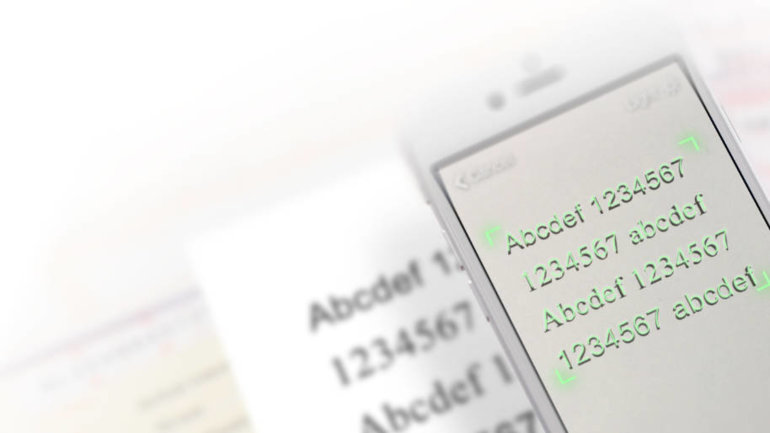
\includegraphics[width=10cm]{images/mobile-ocr.jpg}
    \caption{OCR-sustav na mobilnom uređaju. \citep{Microblink}}
    \label{fig:mobile-ocr}
\end{figure}
\end{frame}

\subsubsection{Primjene optičkog raspoznavanja znakova}
\begin{frame}
\frametitle{Optičko raspoznavanje znakova}
\framesubtitle{Primjene optičkog raspoznavanja znakova (1)}
\begin{itemize}
    \item Bankovne aplikacije za mobilne uređaje
    \begin{itemize}
        \item Plaćanje računa
        \item Otvaranje bankovnog računa (npr. Zagrebačka banka, Revolut, N26)
    \end{itemize}
    \item Turizam i hoteljerstvo
    \begin{itemize}
        \item Prijava boravka u hotelima
    \end{itemize}
    \item Registracija glasovanja na biralištima
    \item Registracija posjetitelja na raznim događajima
    \item Granične kontrole
    \item Upravljanje financijama
    \item Digitalizacija knjiga
    \item Detekcija znakova na registarskim pločicama
\end{itemize}
\end{frame}

\begin{frame}
\frametitle{Optičko raspoznavanje znakova}
\framesubtitle{Primjene optičkog raspoznavanja znakova (2)}
\begin{figure}[htb]
    \centering
    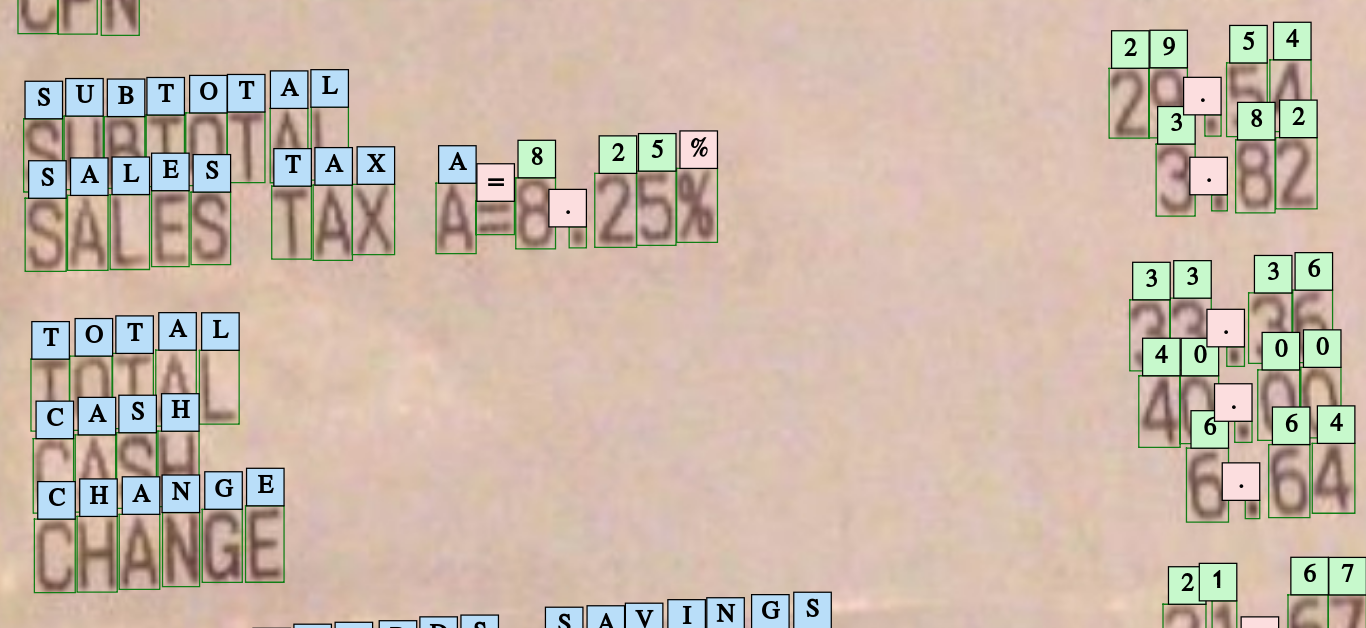
\includegraphics[width=12cm]{images/receipt-example-01.png}
    \caption{Vizualizacija rezultata OCR-sustava.}
    \label{fig:ocr-result-01}
\end{figure}
\end{frame}

\subsubsection{Komponente sustava za optičko raspoznavanje znakova}
\begin{frame}
\frametitle{Optičko raspoznavanje znakova}
\framesubtitle{Komponente sustava za optičko raspoznavanje znakova}
Optičko raspoznavanje znakova provodi se u nekoliko koraka:
\begin{itemize}
    \item pribavljanje slike,
    \item predobrada,
    \item segmentacija znakova,
    \item izdvajanje značajki znakova,
    \item klasifikacija znakova i
    \item \textbf{naknadna obrada}.
\end{itemize}
\end{frame}

\section{Određivanje strukture teksta na temelju položaja pojedinih znakova}
\subsection{Željena funkcionalnost}
\begin{frame}
\frametitle{Određivanje strukture teksta na temelju položaja pojedinih znakova}
\framesubtitle{Željena funkcionalnost}
\begin{figure}[htb]
    \centering
    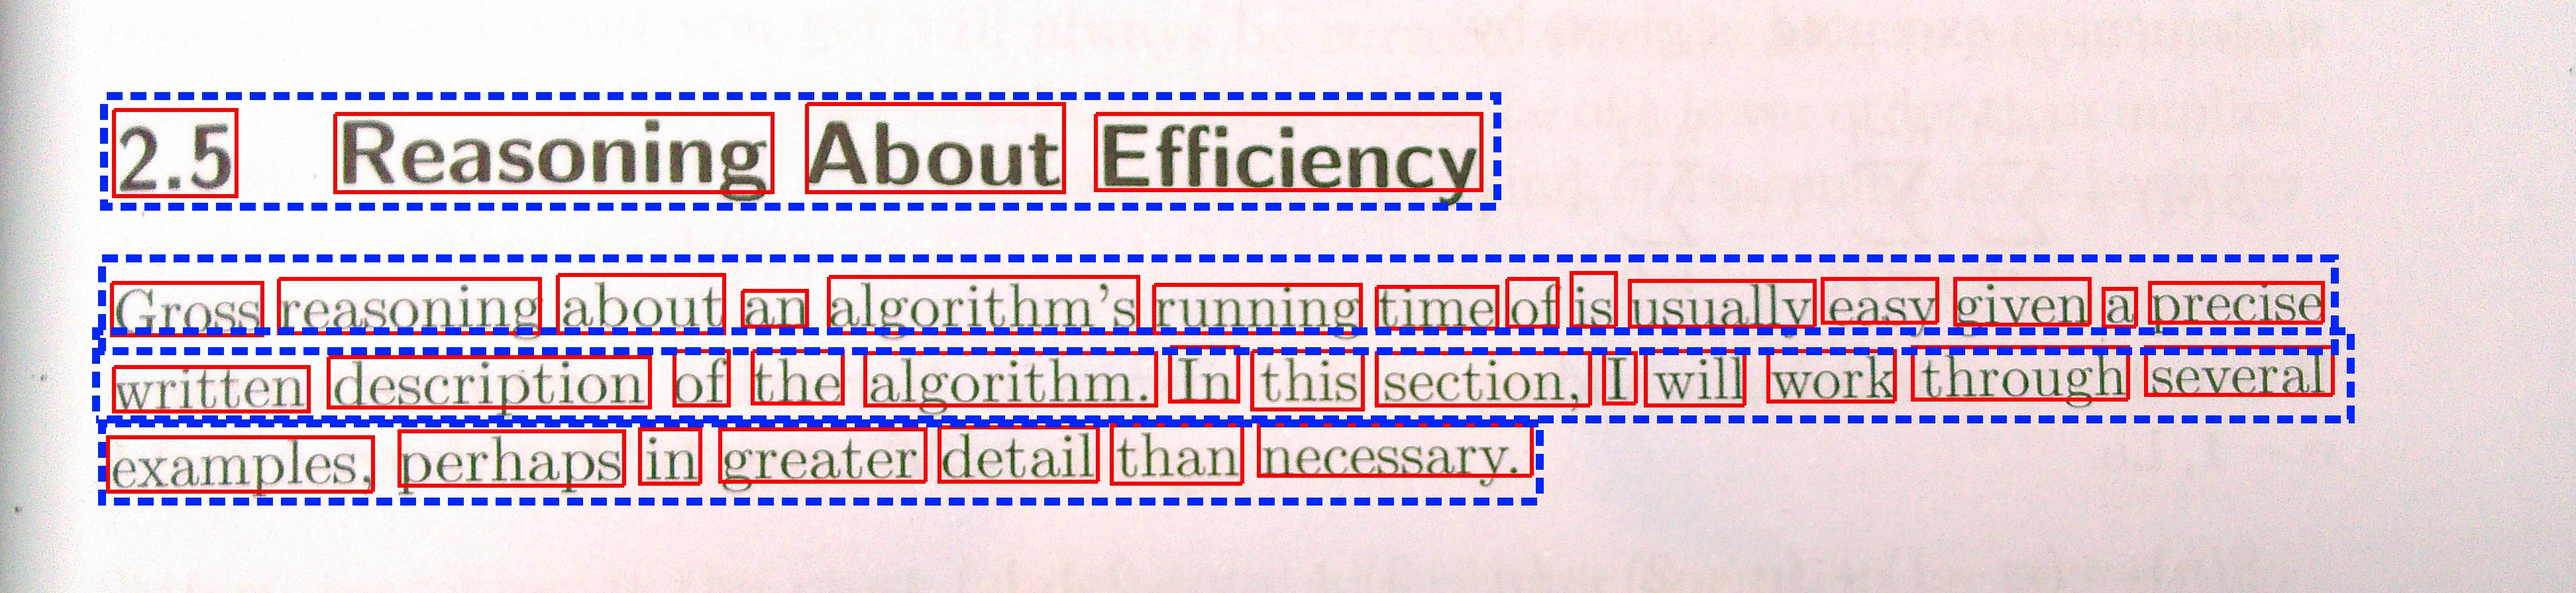
\includegraphics[width=\textwidth]{images/text-segmentation-01.jpg}
    \caption{Vizualizacija rezultata sustava za određivanje strukture teksta.}
    \label{fig:text-segmentation-01}
\end{figure}
\end{frame}

\subsection{Suradnja s OCR-sustavom}
\begin{frame}
\frametitle{Određivanje strukture teksta na temelju položaja pojedinih znakova}
\framesubtitle{Suradnja s OCR-sustavom}
\begin{figure}[htb]
    \centering
    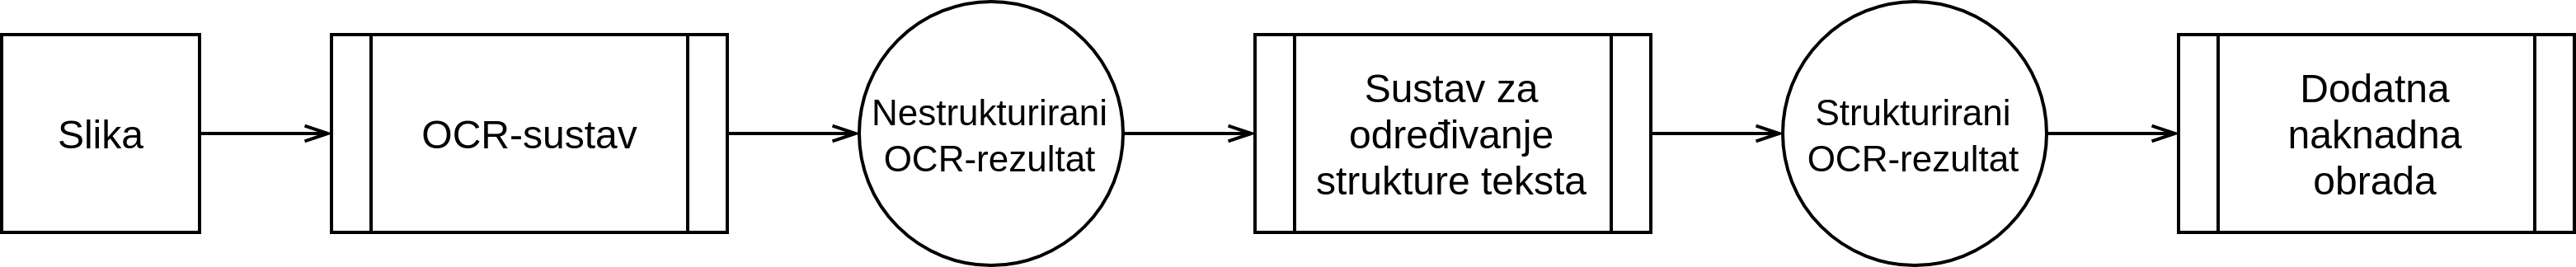
\includegraphics[width=\textwidth]{images/sustav-01.png}
    \caption{Suradnja OCR-sustava i sustava za određivanje strukture teksta.}
    \label{fig:sustav-01}
\end{figure}
\end{frame}

\subsection{Skup podataka za ispitivanje}
\begin{frame}
\frametitle{Određivanje strukture teksta na temelju položaja pojedinih znakova}
\framesubtitle{Skup podataka za ispitivanje}
Skup podataka za ispitivanje sastoji se od:
\begin{itemize}
    \item slika,
    \item ulaznih datoteka u formatu JSON i
    \item očekivanih izlaznih datoteka
\end{itemize}
\end{frame}
\begin{frame}
\frametitle{Skup podataka za ispitivanje}
\framesubtitle{Slike (1)}
\begin{itemize}
    \item \textbf{Ručno} označene i klasificirane slike
    \item 100 slika računa iz trgovina (ukupno 85068 znakova)
    \item 34 slike sadržaja iz knjiga (ukupno 25092 znaka)
\end{itemize}
\begin{figure}[htb]
    \centering
    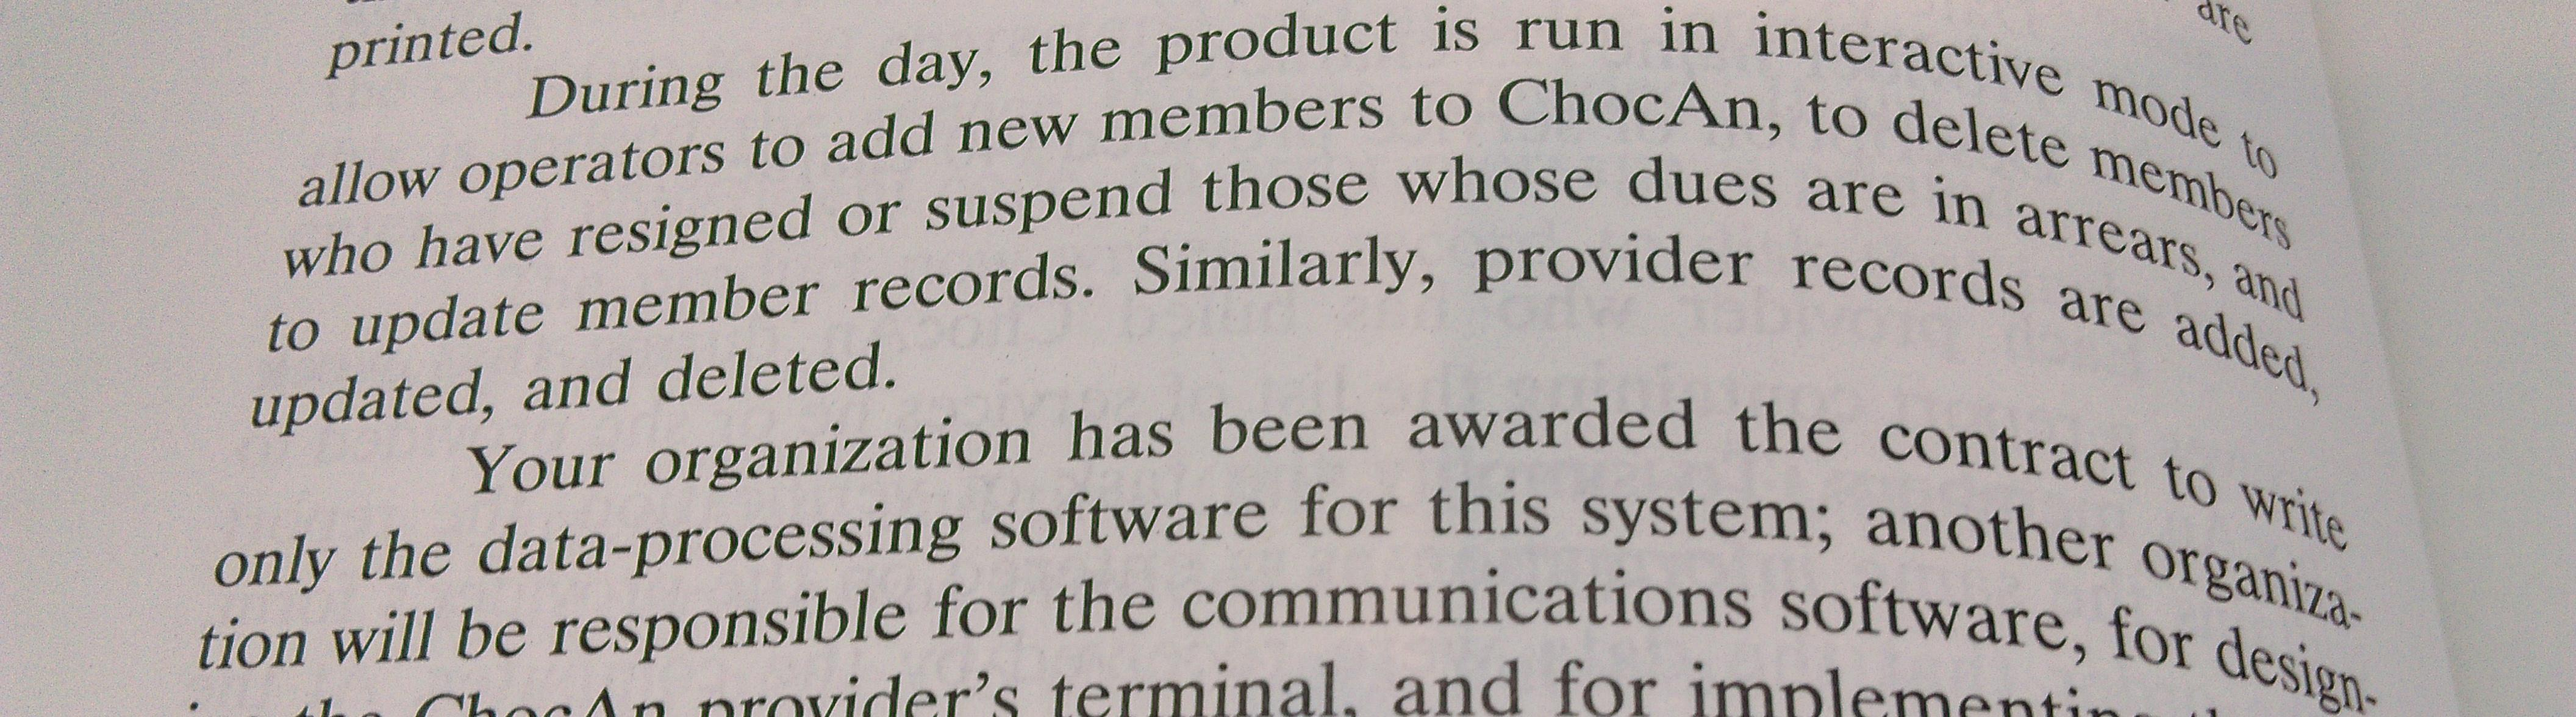
\includegraphics[width=\textwidth]{images/book-example-03.jpg}
    \caption{Primjer slike sadržaja iz knjige.}
    \label{fig:book-example-04}
\end{figure}
\end{frame}
\begin{frame}
\frametitle{Skup podataka za ispitivanje}
\framesubtitle{Slike (2)}
\begin{figure}[htb]
    \centering
    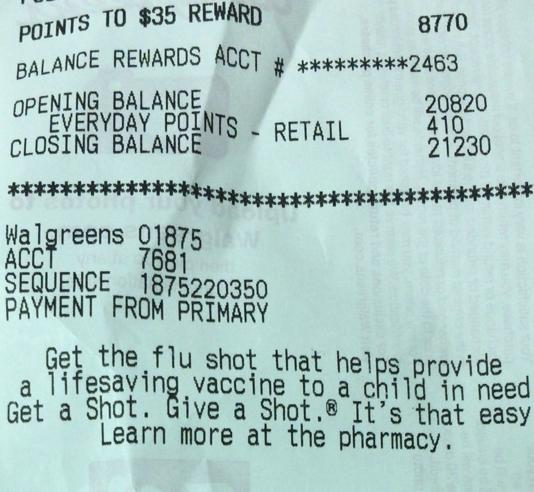
\includegraphics[width=7cm]{images/receipt-example-04.jpg}
    \caption{Primjer slike računa iz trgovine.}
    \label{fig:receipt-example-04}
\end{figure}
\end{frame}
\begin{frame}
\frametitle{Skup podataka za ispitivanje}
\framesubtitle{Slike (3)}
\begin{figure}[htb]
    \centering
    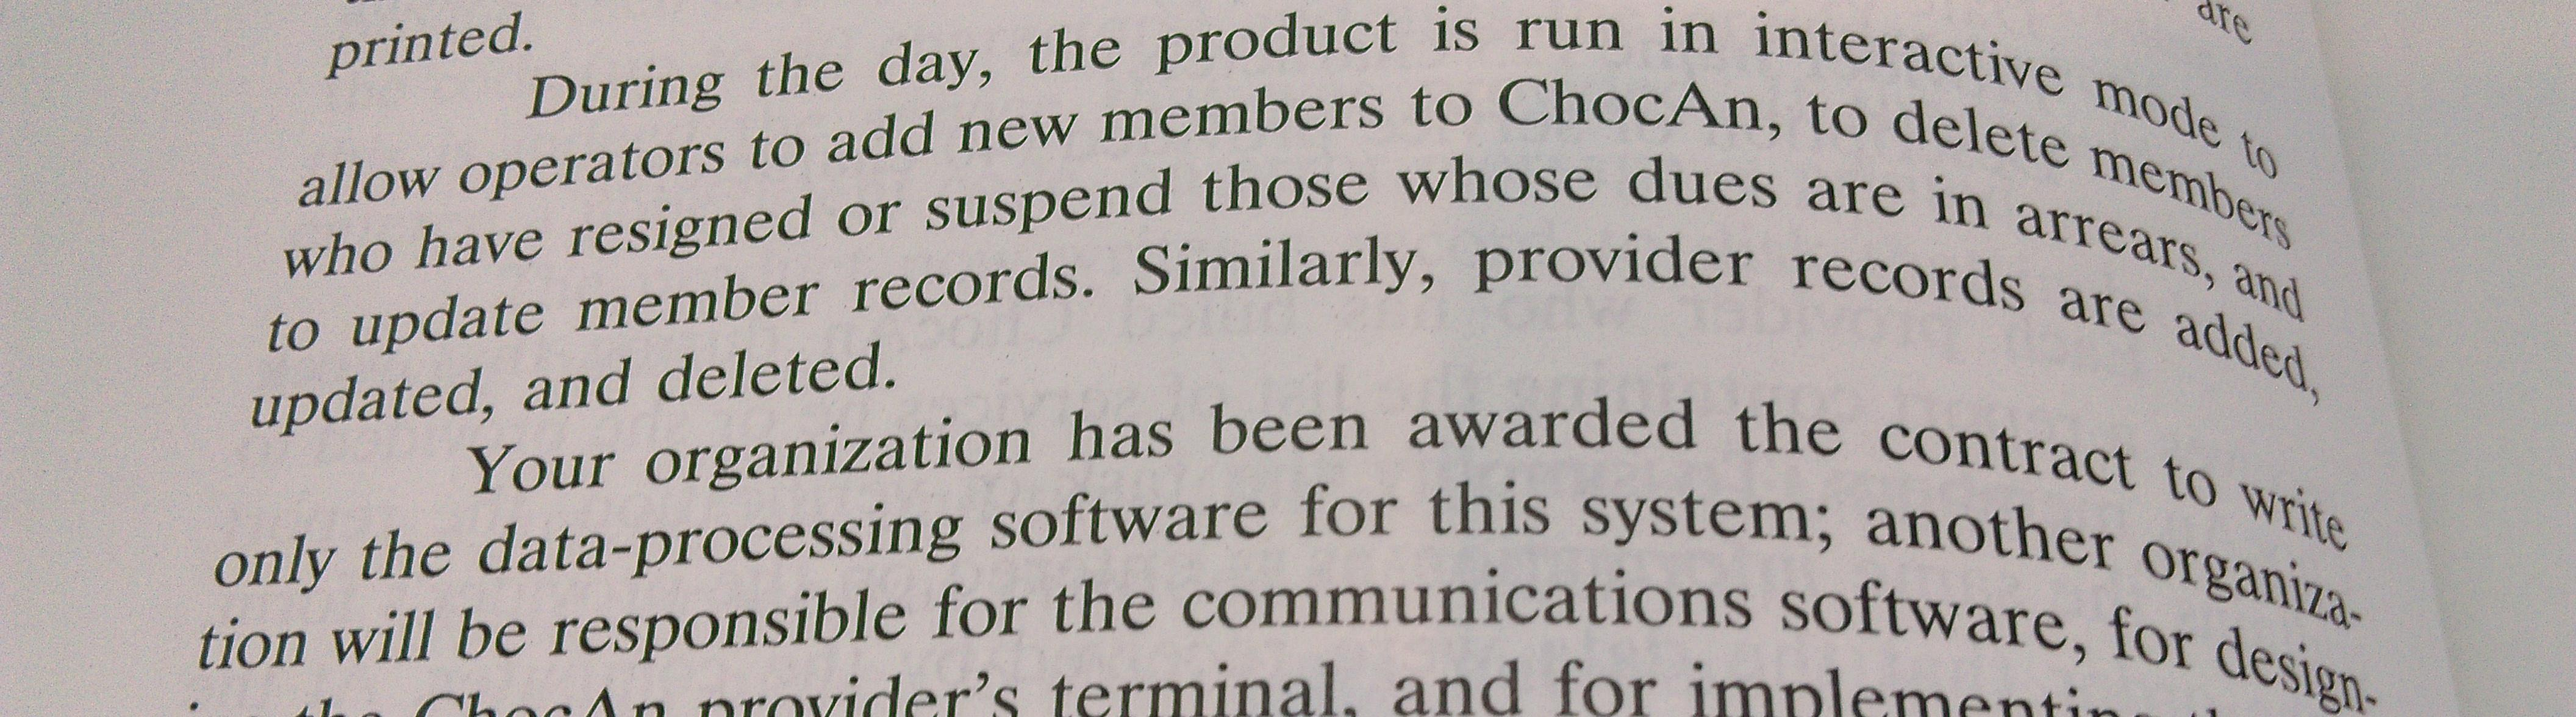
\includegraphics[width=\textwidth]{images/book-example-03.jpg}
    \caption{Primjer slike s ukošenim tekstom.}
    \label{fig:book-example-03}
\end{figure}
\end{frame}


\subsection{Korištenje skupa podataka za ispitivanje}

\section{Algoritmi za određivanje strukture teksta}
\subsection{Algoritmi za određivanje linija}

\subsection{Algoritmi za rastavljanje riječi}

\section{Mjere točnosti algoritama}
\section{Rezultati}
\section{Zaključak}

\begin{frame}
\frametitle{Literatura}
\bibliography{literatura}
\bibliographystyle{fer}
\end{frame}

\end{document}
